\documentclass[journal]{IEEEtran}
\usepackage{amssymb}
\usepackage{lineno}
\usepackage{fixltx2e}
\usepackage{hyperref}
\usepackage{enumitem}
\usepackage{amsmath}
\usepackage{graphicx}
\usepackage{listings}
\usepackage{tabularx}
\usepackage{float}
\usepackage{pbox}
\usepackage{xcolor}
\usepackage[hang, small,labelfont=bf,up,textfont=it,up]{caption} % Custom captions under/above floats in tables or figures
\usepackage{booktabs} % Horizontal rules in tables
\usepackage{microtype} % Slightly tweak font spacing for aesthetics
\usepackage[english]{babel} % Language hyphenation and typographical rules
\usepackage[normalem]{ulem}
\useunder{\uline}{\ul}{}

\lstset{ %
	language=C,                % choose the language of the code
	basicstyle=\footnotesize,       % the size of the fonts that are used for the code
	numbers=none,                   % where to put the line-numbers
	numberstyle=\footnotesize,      % the size of the fonts that are used for the line-numbers
	stepnumber=1,                   % the step between two line-numbers. If it is 1 each line will be numbered
	backgroundcolor=\color{white},  % choose the background color. You must add \usepackage{color}
	showspaces=false,               % show spaces adding particular underscores
	showstringspaces=false,         % underline spaces within strings
	showtabs=false,                 % sh-ow tabs within strings adding particular underscores
	frame=single,           % adds a frame around the code
	tabsize=2,          % sets default tabsize to 2 spaces
	captionpos=b,           % sets the caption-position to bottom
	breaklines=true,        % sets automatic line breaking
	breakatwhitespace=false,    % sets if automatic breaks should only happen at whitespace
	escapeinside={\%*}{*)}          % if you want to add a comment within your code
}

\DeclareMathOperator*{\argmax}{arg\,max}

\begin{document}
	
\title{Comparing five common classification algorithms on the ORL and MNIST data set}

%% use optional labels to link authors explicitly to addresses:
%% \author[label1,label2]{<author name>}
%% \address[label1]{<address>}
%% \address[label2]{<address>}

\author{Christian~M.~Lillelund,~\IEEEmembership{201408354@post.au.dk,~School of Engineering, Aarhus University}
\thanks{Report revised December 10, 2018.}}
\maketitle

%\address{School of Engineering, Aarhus University}

%\address{X}

\begin{abstract}
Today's computer systems offer a significant potential for training and testing machine learning techniques and classification algorithms, however the choice of algorithm depend on the problem at hand, one's amount of train and test data and the computational resources at one's disposal. In this report we review one dimensionality reduction technique and five common classification schemes and evaluate their performance on the ORL (human faces) and MNIST (hand-written numbers) data set. We find that simple algorithms like the Nearest Neighbor classifier work great performance and accuracy wise when training on the small data set, ORL, but struggle to keep up with more complex algorithms like a Perceptron using backpropagation on the large set, MNIST, as the dimensionality and amount of samples is significantly increased.
\end{abstract}

\begin{IEEEkeywords}
	IEEE, IEEEtran, journal, \LaTeX, paper, template.
\end{IEEEkeywords}

\section{Introduction}
For humans, it does not take much effort to tell the difference between a picture of a dog or a cat. A natural number or a letter. A happy person or a sad person. For computers, these sort of problems are notorious hard to solve and often require many computational resources\footnote{\cite{TerenceMills2018}}. Machine learning and computer vision deals with these issues as they encompass a range of algorithms and classification techniques to produce a model or scheme that can tell images apart and recognize similarities. In this report we study the recognition and classification of a data set containing human faces and one featuring hand-written numbers by implementing and testing five commonly used techniques (Nearest class centroid classifier, nearest sub-class centroid, nearest neighbor and two perceptron variants) using MATLAB. We split the data in a training and a test set, then train our respective classifier and evaluate its ability to classify correctly on the testing set. A version using all the dimensions of the training data samples and a principal component version will be applied. We use some MATLAB visualization techniques to better communicate the data representation and tables to compare them. We start by going over the basic theory behind the classification schemes, then look at the data, briefly go over implementation details and then turn to results. At the end we review and argue which scheme would make the most sense to use with these two classification problems.

Initially, we split the ORL image data set, containing 400 40x30 pixel faces of 40 different persons, and the MNIST set containing 70.000 28x28 pixel hand-written numbers from zero to nine. The data is vectorized, so we use built-in MATLAB functions to construct the original pictures as such:

\begin{figure}[h]
	\centering
	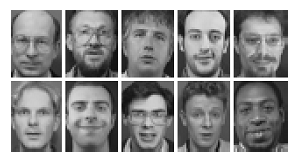
\includegraphics[width=0.7\linewidth]{orlfaces}
	\caption{Ten random images of faces from the ORL set.}
	\label{fig:orlfaces}
\end{figure}

\begin{figure}[h]
	\centering
	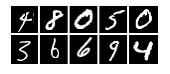
\includegraphics[width=0.7\linewidth]{mnistnumbers}
	\caption{Ten random images of numbers from the MNIST set.}
	\label{fig:mnistnumbers}
\end{figure}

\section{Theory}
This section will explain fundamental theory behind the dimensional reduction technique (PCA) and the five schemes used in this report.

\subsection{Principal Component Analysis}

PCA is a procedure that transform a set of observations or samples in dimension $D$ to a lower dimension $D-n$ while still preserving a smaller number of variables explaining the main features $X_{1}, X_{2}, ..., X_{p}$ in the original set\footnote{\cite{Casella}}. This is particularly useful when dealing with high dimension data, as this can be computationally hard and challenging to visualize. With PCA, we compute principal components $d$ of $n$ original samples with $p$ features, where $d$ is the desired output dimensionality and each dimension is a linear combination of the $p$ features. In practice, we find eigenvectors of the covariance matrix of the original data set, sort them by highest eigenvalue score and use these as weights $W$ in computing a linear transformation: $$y_{i} = W^T*x_{i}, i = 1, ..., N$$. The scattering of the transformed data is the scatter matrix given by \footnote{\cite{Iosifidis2017}}: $$S_{T} = \sum_{i=1}^{N} [W^T(x_{i}-\mu)][W^T(x_{i}-\mu)]^T$$. The weights $W$ can be found by applying eigenanalysis and taking the eigenvectors with the  highest score, more formally optimizing \footnote{\cite{Iosifidis2017}}: \[ W^* = \argmax_c Tr (W^TS_{T}) \] subject to $W^TW=I$. We end with a data set containing fewer ($d < D$) dimensions.

\subsection{Nearest class centroid classifier}

The NCC classifier assigns labels $l_{i}$ to $N$ observations determined by which class $c_{k}$'s mean (centroid) the observation $x_{i}$ is closest to. We make the assumption that each class follow a normal distribution, as they are given equal importance in the classification algorithm. The mean class vector is given by \footnote{\cite{Iosifidis2017}}: $$ \mu_{k} = \frac{1}{N_{k}} \sum_{i,li=k}^{} x_{i}, k = 1, ... K.$$

To classify any observation $x_{i}$ we find the smallest distance to any mean vector and assign the label of that vector to $x_{i}$, more formally: $$ d(x_{i},\mu_{k}) = ||x_{i}-\mu_{k}||^2_{2} $$

\subsection{Nearest subclass centroid classifier}

Similar to nearest class centroid, but each class $c_{k}$ now has subclasses $m$ that follow a normal distribution and has a mean vector $\mu_{km}$: $$ \mu_{km} = \frac{1}{N_{km}} \sum_{i,li=k, qi=m}^{} x_{i} $$ where $N_{km}$ denotes the number of observations in a given subclass and $x_{i}$ is a observation with a subclass label $qi$. Like NCC, the distance to the subclass mean is used to classify each observation \footnote{\cite{Iosifidis2017}}: $$ d(x_{i},\mu_{km}) = ||x_{i}-\mu_{km}||^2_{2} $$

The number of subclasses is a hyper parameter for NSC and must be decided prior. Nearest subclass classifier is a compromise between nearest mean and nearest neighbor and combines the flexibility of nearest neighbor with the robustness of nearest mean \footnote{\cite{Veenman2005}}. When the number of subclasses $m$ is equal to $N$ samples, we have the nearest neighbor classifier.

\subsection{Nearest neighbor classifier}

The nearest neighbor (NN) classifier is a simple algorithm where each sample is assigned to the class of its closest neighbor, or the most common class among its $k$ nearest neighbors in the k-NN variant. Pure NN is when $k=1$, but often $k>1$ where a majority vote takes place. The algorithm uses euclidean distance between a test sample $x_{i}$ with class $c_{k}$ and a training one $y_{i}$: $$ d(x_{i},y_{i}) = ||x_{i}-y_{i}||^2_{2} $$

\subsection{Perceptron learning with backpropagation}

A perceptron is a supervised algorithm of binary classifiers, that classify whether or not an input sample $x_{i}$ belong to a class $c_{k}$. It uses the linear discriminant function $f(x) = w^T*x + w_{0}$, where $w$ are weights, $x\varepsilon$ $\mathbb{R^D}$ a feature vector and $w_{0}$ the bias\footnote{\cite{Iosifidis2017}}. $w$ represent the orientation of the discriminant hyperplane, and $w_{0}$ a offset from the origin. Given weights $w$, sample $x_{i}$ and classes $c_{1}$ and $c_{2}$, the function splits the feature space into these two classes. If $g(w,x_{i}) > 0$, $x_{i}$ belongs to $c_{1}$ and if $g(w,x_{i}) < 0$, $x_{i}$ belongs to $c_{1}$. If $g(w,x_{i}) = 0$, it can be classified to either class. The resulting scalar is the distance of $x_{i}$ to the hyperplane. The function is used in our perceptron to follow, where we define a binary label $l_{i}$ for each sample to express the criterion function: $$ f(w^*,x_{i}) = l_{i} g(w,x_{i}) = l_{i} w^{*T} x_{i} \geq 0, i = 1, ..., N $$

All samples are correctly classified, if $f(w_{*}, x_{i}) \geq 0$. To produce such result, we need to optimize weights $w_{*}$ by the perceptron criterion function for $w_{*}$, where ${\jmath}_{p}(w_{*}) = 0$ would be a solution for\footnote{\cite{Iosifidis2017}} $w_{*}$: $$ {\jmath}_{p}(w) = \sum_{x_{i} \varepsilon \chi}^{} -f(w,x_{i}) = \sum_{x_{i} \varepsilon \chi}^{} -l_{i} w^T x_{i} $$

To optimize ${\jmath}_{p}(w)$, we use the gradient at $w$ and follow it to update $w$, where $\eta$ is the rate of change (learning rate) and expresses how fast it converges, and $\varepsilon$ express a vector set of mislabeled samples:

$$ w(t+1) = w(t) - \eta(t) \nabla{\jmath}_{p} = w(t) + \eta(t) \sum_{x_{i} \varepsilon \chi}^{} l_{i} x_{i} $$

At each learning iteration, the weights $w(t)$ are "punished" by the sum of misclassified samples scaled, leading to convergence as the result of criterion function ${\jmath}_{p}$ will be higher. This is known as backpropagation. The algorithm to come will elaborate on this.

\subsection{Perceptron learning with MSE}

As an alternative to backpropagation, one can apply least-mean square regression to obtain the perceptron weights $W$. Here we use a criterion function ${\jmath}_{LSE}$ that involves all of the samples, not just the misclassified ones. Previously we made the inner products of $f(X) = W^T*X$ positive, now we look to find a solution to $W^T X = t_{i}, i = 1, ..., N$, where $t_{i}$ are arbitrarily set positive constants. This is written as $X^T*w = b$ in matrix form. If X is nonsingular, we could write $W = X^-1 b$ and have a formal solution, but this is often not the case, however by obtaining the pseudo-inverse of $X$ one can find a solution for the weights\footnote{\cite{Duda2012}}: $$ X^\dagger = (X^tX)^{-1}X^T $$

Examining the criterion function, we look to minimize: $$ {\jmath}_{LSE} = ||W^T X - B||^2_{F} $$

By setting the derivative of this to zero with respect to $W$, we get: $$ \nabla{\jmath}_{LSE} = 0 => 2XX^W = 2XB^T $$

Hence: $$ W = (XX^T)^{-1} XB^T = W^\dagger B^T $$

If W is square and nonsingular, the pseudo-inverse is simply the regular inverse. Also it holds at $X^\dagger X = I$, but $X X^\dagger \neq I$, though a MSE always exists, hence $W = X^\dagger b$ is an MSE solution to $X^\dagger w = b$.

\section{Implementation}

The implementation uses MATLAB to design and run the different schemes on the training and test data. For understanding purposes, this section will briefly lay out the algorithms described in theory as pseudo-code.

\subsection{PCA} 

The algorithm centers the data, then simply calculates eigenvectors from the variance matrix, sort them after highest eigenvalue and uses the $n$ vector as a principal component in representing the data. Listing \ref{lst:pca} shows the PCA as pseudo-code.

\begin{lstlisting}[caption=Implementation of PCA., label={lst:pca}, belowskip=-0.8 \baselineskip]
	pca_reduce(trainData, nDimensions) {
		trainData = trainData - mean(trainData) for rows in trainData
		eigVectors, eigValues = eig(cov(trainData))
		eigVectors = sort(eigVectors, 'descending')
		pc = eigVectors(from 1 to nDimensions)*trainData
	}
\end{lstlisting}

\subsection{NCC} 

NCC simply calculates a mean vector for $c_{k}$ classes by summing the samples that belong to the class and dividing that with the number of $N$ samples in a given class, as expressed in listing \ref{lst:ncc}.

\begin{lstlisting}[caption=Implementation of NCC., label={lst:ncc}]
	train_ncc(trainData, trainLbls, nClasses) {
		mu = zero vector by size of trainData*nClasses
		n = zero vector by size of 1*nClasses
		index = 1;
		
		for (i = 1; i <= nClasses;i++) {
			n(i) = sum(num of classes i in trainLbls)
			mu(i) = sum(each traning sample from index to n(i))/n(i)		
			index = index+n(i)
		}
	}
\end{lstlisting}

\subsection{NSC} 

NSC makes an initial k-means clustering of the training data for $k=m$ subclasses as hyper parameter and use the resulting centroids to construct a new centroid matrix for each subclass $m$ spanning $c_{k}$*$m$. Listing \ref{lst:nsc} shows this.

\begin{lstlisting}[caption=Implementation of NSC., label={lst:nsc}]
	train_nsc(trainData, trainLbls, nClasses, nSubClasses) {
		centroids = zero vector by size of trainData*(nClasses*nSubClasses)
		n = zero vector by size of 1*nClasses
		index = 1;
		centroidIdx = vector to keep idx of centroids
	
		for (i = 1; i <= nClasses;i++) {
			n(i) = sum(num of classes i in trainLbls)
			[idx,clst] = kmeans(trainData for index+n(i), nSubClasses)
			centroids(for idx in centroidIdx) = clst
			index = index+n(i)-1
		} }
\end{lstlisting}

\subsection{NNC}

The algorithm takes as input the training and test data, as well as training labels. It then iterates through every test sample $x_i$ and compares to every single training sample $X_{i}$. It classifies $x_i$ to the class of $X_{i}$ it is closest too in Euclidean distance. Listing \ref{lst:nnc} shows this.

\begin{minipage}[H]{0.95\linewidth}
	\begin{lstlisting}[caption=Implementation of NNC., label={lst:nnc}]
	train_nnc(trainData, trainLbls, testData) {
		distances = zero vector by size testData*trainData
		resultLabels = zero vector by size testData*1
		nTestImages = num of test images
		nTrainImages = num of train images
		
		for (i = 1; i <= nTestImages; i++) {
			for (j = 1; j <= nTrainImages; j++) {
				distances(i,j) = norm(testData(i)-trainData(j), 2)^2.
			}			
			trainIndex = min(distances(i))
			resultLabels = trainLbls(trainIndex)
		}
	\end{lstlisting}
\end{minipage}

\subsection{Perceptron with backpropagation} 

The algorithm trains a perceptron to correctly classify each sample $x_{i}$ to class $c_{k}$. We start with an empty vector $\chi$, then create a label $l_{i}$ for sample $x_{i}$ setting it to 1 if it corresponds to our current class, otherwise -1. We then use a one-vs-rest criterion function $f(w,x)$ for the $x_{i}$'s, save the wrongly classified samples and labels, then summing the wrong samples times their label and use this value to update weights $w_{k}$ iteratively. The learning eta $\eta$ is a hyper parameter. Listing \ref{lst:pbp} shows the pseudo-code for this.

\begin{lstlisting}[caption=Implementation of a perceptron with backprogapation., label={lst:pbp}]
	train_perp_bp(trainData, trainLbls, eta, nClasses) {
	w = random W matrix with size trainData*nCLasses
	maxIters = max itertions
	for (k = 1; k <= nClasses; k++) {
		wrongLabels = empty matrix to save labels
		done = false, i = 0
		while (not done and nIters < maxIters) {
			X = empty matrix for wrong x_i's
			for (i = 1; i <= nTrainImages, i++) {
				x_i = trainData(i)
				if(trainlbls(i) = k) label = 1 else label = -1
				if (label*w(k)*x_i) < 0
					save x_i to X, save label to WrongLabels
			}
			sumOfWrongs = sum(WrongLabels * X)
			w(k) = w(k) + eta * sumOfWrongs
			ifEmpty(X)
				done = true
			}
		}
	}
\end{lstlisting}

\subsection{Perceptron with MSE} 

The algorithm for MSE is simplified, but possibly more computational demanding. We start by finding the pseudo-inverse of our training data set, then create a label vector for each class $c_{k}$ with $l_{i} = 1$ if the label is in the class or $l_{i} = -1$ if it is not. Finally we find the MSE solution by multiplying the two for weight $W_{k}$. Listing \ref{lst:pmse} shows this.

\begin{lstlisting}[caption=Implementation of NSC., label={lst:pmse}]
	train_perp_mse(trainData, trainLbls, nClasses) {
		w = random W matrix with size trainData*nCLasses
		X = pseudo-inverse of trainData
		
		for (k = 1; k <= nClasses; k++) {
			Labels = empty matrix to save labels
			for (i = 1; i <= nTrainImages; i++)
				if (trainlbls(i) = k)
					save 1 to Labels
				else save -1 to Labels
			}
			w(:,k) = X*Labels;
		}
	}
\end{lstlisting}

\section{Results}

The five classification schemes are trained and tested on the ORL and MNIST data set with scatter plots to visualize the resulting labels compared to the testing ones and a confusion matrix that depicts the predicated and true classes. Each algorithm is tested with both the PCA and the full version of the data. All results were done with MATLAB R2018a on an Intel i5 4690K @ 3.50Ghz CPU. We start by showing the output of the PCA analysis, and then proceed to the classifications.

\subsection{PCA}

PCA was performed on both ORL and MNIST data set for number of dimensions $D=2$ with MATLAB. Table \ref{table:pca} details the computation time for PCA and figure \ref{fig:orlpca} and \ref{fig:mnistpca} shows a scatter plot with two principal components, i.e. the eigenvectors with highest eigenvalues.

\begin{table}[H]
	\centering
	\begin{tabular}{|l|l|l|l} \hline
		Data set & \pbox{18cm}{Method} & \pbox{5cm}{Execution time in $s$} \\ \hline
		ORL & PCA & 0.33 \\ \hline
		MNIST & PCA & 0.83 \\ \hline
	\end{tabular}
	\caption{PCA on ORL and MNIST data set.}
	\label{table:pca}
\end{table}

\begin{figure}[H]
	\centering
	\frame{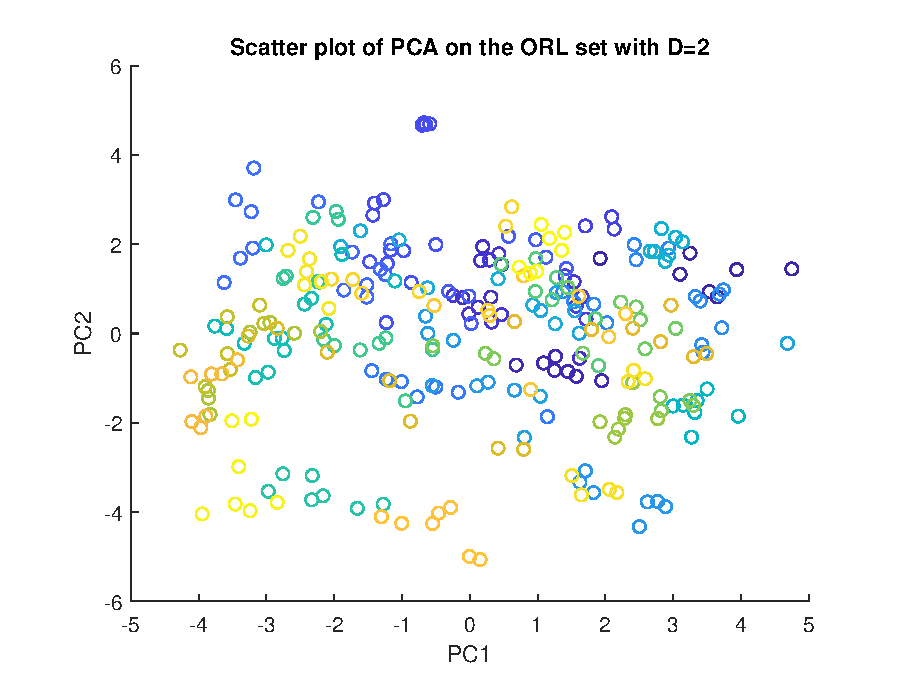
\includegraphics[width=0.7\linewidth]{../ML/results/ORL_PCA}}
	\caption{Plot of two PC's on ORL. Data labels are colors.}
	\label{fig:orlpca}
\end{figure}

\begin{figure}[H]
	\centering
	\frame{\includegraphics[width=0.7\linewidth]{../ML/results/MNIST_PCA}}
	\caption{Plot of two PC's on MNIST. Data labels are colors.}
	\label{fig:mnistpca}
\end{figure}

\subsection{NCC}

Nearest Centroid was conducted on ORL and MNIST. To test the algorithm, we find the class $c_{k}$'s mean to which a sample $x_{i}$ is closest to by calculating the Euclidean distance (L2-norm) between a test sample and the mean vector. Table \ref{table:ncc} details performance and accuracy, while figure \ref{fig:orlnc} and \ref{fig:mnistnc} shows the resulting labels on scatter plots. The tests were performed on full-dimensional sets and PCA reduced sets. Accuracy is the number of resulting labels that equal the testing labels divided by the number of test samples.

\begin{table}[H]
	\centering
	\begin{tabular}{|l|l|l|} \hline
		Data set & \pbox{18cm}{Accuracy in $\%$} & \pbox{18cm}{Execution time in $s$} \\ \hline
		ORL & 94,1\% & 0.00 \\ \hline
		ORL w. PCA & 15,8\% & 0.00 \\ \hline
		MNIST & 75,2\% & 0.34 \\ \hline
		MNIST w. PCA & 14,9\% & 0.00 \\ \hline
	\end{tabular}
	\caption{Results for NCC performed on ORL and MNIST.}
	\label{table:ncc}
\end{table}

\begin{figure}[H]
	\centering
	\frame{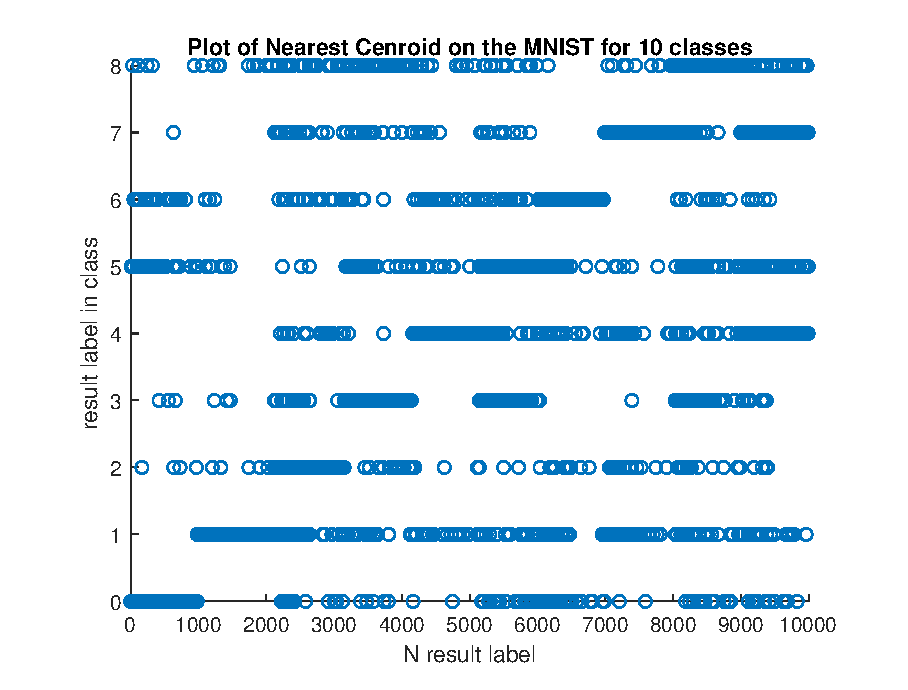
\includegraphics[width=0.6\linewidth]{../ML/results/ORL_NC}}
	\caption{Plot results of NCC on ORL.}
	\label{fig:orlnc}
\end{figure}


\begin{figure}[H]
	\centering
	\frame{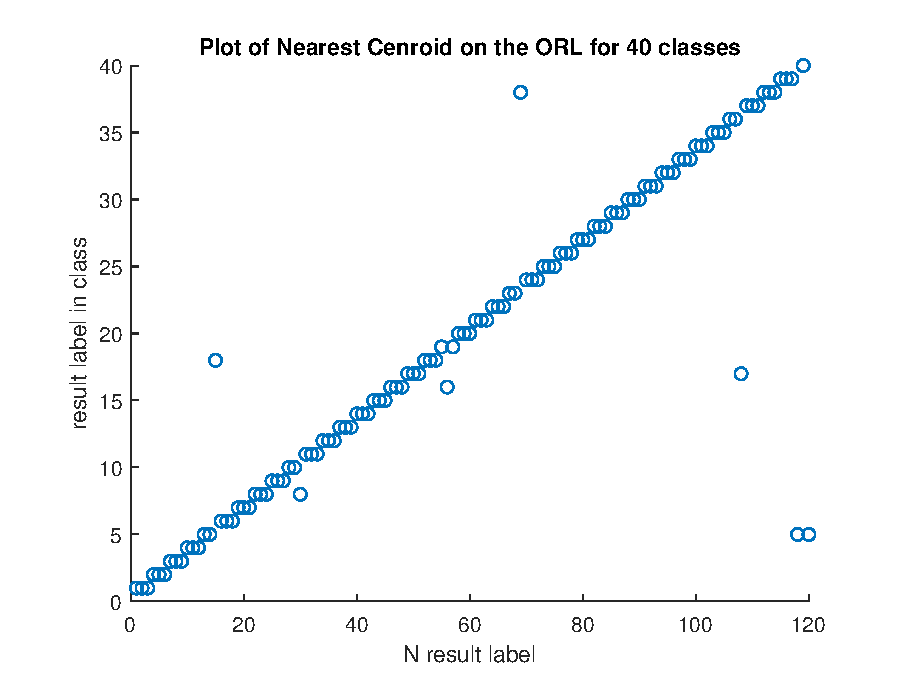
\includegraphics[width=0.6\linewidth]{../ML/results/MNIST_NC}}
	\caption{Plot results of NCC on MNIST.}
	\label{fig:mnistnc}
\end{figure}

\subsection{NSC}

Nearest Subclass Centroid was performed on ORL and MNIST with hyper-parameter $N_{sc}=2, N_{sc}=3, N_{sc}=5$ for number of subclasses. Our algorithm returns centroids for number of classes $N_{c}=N_{ck}*N_{sc}$. We classify a testing sample to a class of which its centroid it is closest to. Table \ref{table:nsc} details the result. $N_{sc}$ is number of subclasses. Figure \ref{fig:orlnsc} and \ref{fig:mnistnsc} show the NSC on the ORL and MNIST data set. The blue color represents test labels, the red color represents result labels. Each test sample is plotted to their class.

\begin{table}[H]
	\centering
	\begin{tabular}{|l|l|l|l|} \hline
		Data set & \pbox{18cm}{$N_{sc}$} & \pbox{18cm}{Accuracy in $\%$} & \pbox{18cm}{Execution time in $s$} \\ \hline
		ORL & 2 & 93.3 & 0.15 \\ \hline
		ORL & 3 & 95 & 0.15 \\ \hline
		ORL & 5 & 95.8 & 0.15 \\ \hline
		ORL w. PCA & 2 & 9.1 & 0.13 \\ \hline
		MNIST & 2 & 86.1 & 4.07 \\ \hline
		MNIST & 3 & 88 & 5.99 \\ \hline
		MNIST & 5 & 90 & 9.21 \\ \hline
		MNIST w. PCA & 2 & 14.3 & 0.14 \\ \hline
	\end{tabular}
	\caption{Results for NSC performed on ORL and MNIST.}
	\label{table:nsc}
\end{table}

\begin{figure}[H]
	\centering
	\frame{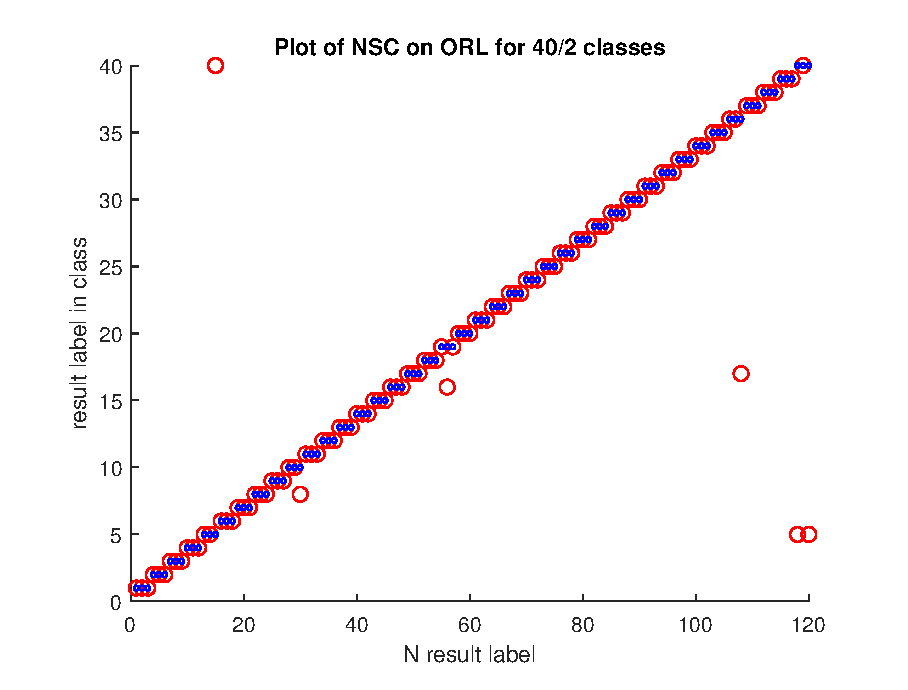
\includegraphics[width=0.6\linewidth]{../ML/results/ORL_NSC}}
	\caption{Plot results of NSC on ORL with $N_{sc}=2$.}
	\label{fig:orlnsc}
\end{figure}

\begin{figure}[H]
	\centering
	\frame{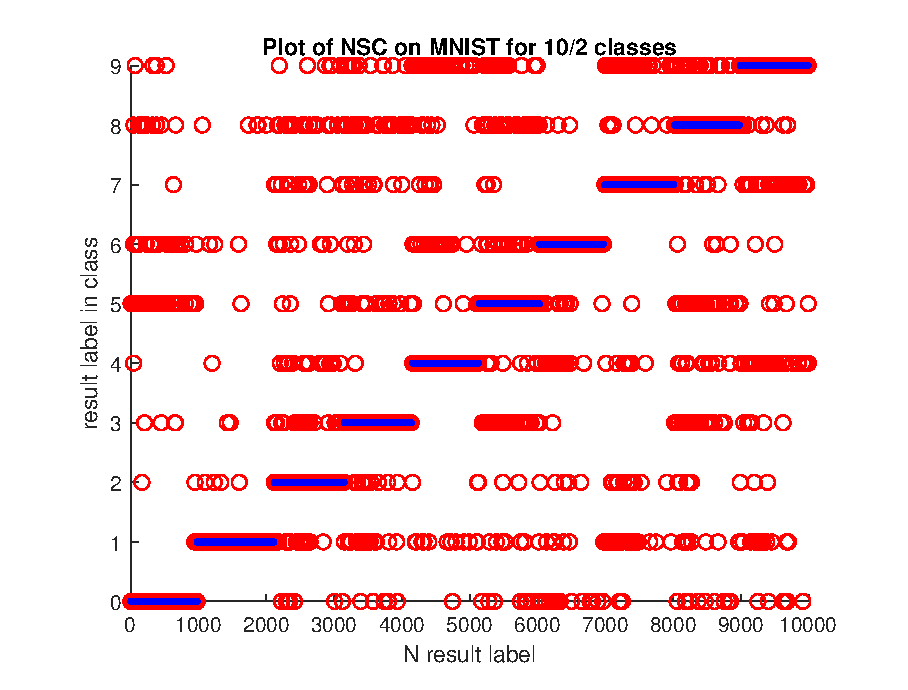
\includegraphics[width=0.6\linewidth]{../ML/results/MNIST_NSC}}
	\caption{Plot results of NSC on MNIST with $N_{sc}=2$.}
	\label{fig:mnistnsc}
\end{figure}

\subsection{NNC}

Nearest Neighbor classifier was performed on ORL and MNIST. To classify a test sample, the algorithm calculates the Euclidean distance to every training sample and assigns the test to whichever training sample it is closest to. Table \ref{table:nn} shows the results with accuracy and execution times. Table \ref{table:nnconfusion} is a confusion matrix to visualize the classification result. It shows samples known to be in class $c_{k}$ classified correctly to $c_{k}$, i.e. 973 samples were rightly classified to class 1.

\begin{table}[H]
	\centering
	\begin{tabular}{|l|l|l|} \hline
		Data set & \pbox{18cm}{Accuracy in $\%$} & \pbox{18cm}{Execution time in $s$} \\ \hline
		ORL & 95.8\% & 0.04 \\ \hline
		ORL w. PCA & 11.6\% & 0.01 \\ \hline
		MNIST & 96.9\% & 676.07 \\ \hline
		MNIST w. PCA & 14.9\% & 264.65 \\ \hline
	\end{tabular}
	\caption{Results of NNC performed on ORL and MNIST.}
	\label{table:nn}
\end{table}

\begin{table}[H]
	\centering
	\begin{tabular}{|l|l|l|l|l|l|l|l|l|l|l|} \hline
		{\ul }      & \textbf{1} & \textbf{2} & \textbf{3} & \textbf{4} & \textbf{5} & \textbf{6} & \textbf{7} & \textbf{8} & \textbf{9} & \textbf{10} \\ \hline
		\textbf{1}  & 973        & 1          & 1          & 0          & 0          & 1          & 3          & 1          & 0          & 0           \\
		\textbf{2}  & 0          & 1129       & 3          & 0          & 1          & 1          & 1          & 0          & 0          & 0           \\
		\textbf{3}  & 7          & 6          & 992        & 5          & 1          & 0          & 2          & 16         & 3          & 0           \\
		\textbf{4}  & 0          & 1          & 2          & 970        & 1          & 19         & 0          & 7          & 7          & 3           \\
		\textbf{5}  & 0          & 7          & 0          & 0          & 944        & 0          & 3          & 5          & 1          & 22          \\
		\textbf{6}  & 1          & 1          & 0          & 12         & 2          & 860        & 5          & 1          & 6          & 4           \\
		\textbf{7}  & 4          & 2          & 0          & 0          & 3          & 5          & 944        & 0          & 0          & 0           \\
		\textbf{8}  & 0          & 14         & 6          & 2          & 4          & 0          & 0          & 992        & 0          & 10          \\
		\textbf{9}  & 6          & 1          & 3          & 14         & 5          & 13         & 5          & 4          & 920        & 5           \\
		\textbf{10} & 2          & 5          & 1          & 6          & 10         & 5          & 1          & 11         & 1          & 967 \\ \hline   
	\end{tabular}
	\caption{Confusion matrix for a NNC model tested on MNIST.}
	\label{table:nnconfusion}
\end{table}

\subsection{Perceptron with BP}

A perceptron was trained on both data sets with the learning rate $\eta$ as hyper-parameter for $\eta=0.01$, $\eta=0.1$, $\eta=1$ and $\eta=10$. For each test sample, we calculate the decision function $y = w(k)*x_{i}$ for each class $c_{k}$ and classify it to the class with maximizes the function. A maximum number of iterations per class is set to 100. Table \ref{table:perceptronbp} details the results, figure \ref{fig:orlperceptronbp} and \ref{fig:mnistperceptronbp} show plots of the resulting labels and \ref{fig:mnistperceptronlinebp1dpca} and \ref{fig:mnistperceptronlinebp2dpca} show the classification perceptron line in 1D and 2D with PCA.

\begin{table}[H]
	\centering
	\begin{tabular}{|l|l|l|l|} \hline
		Data set & \pbox{18cm}{$\eta$} & \pbox{18cm}{Accuracy in $\%$} & \pbox{18cm}{Execution time in $s$} \\ \hline
		ORL & 0.01 & 86.6 & 1.39 \\ \hline
		ORL & 0.1 & 84.1 & 1.30 \\ \hline
		ORL & 1 & 82.5 & 1.36 \\ \hline
		ORL & 10 & 84.1 & 1.34 \\ \hline
		ORL w. PCA & 0.1 & 4.1 & 1.13 \\ \hline
		MNIST & 0.01 & 87.3 & 131.39 \\ \hline
		MNIST & 0.1 & 86.6 & 115.50 \\ \hline
		MNIST & 1 & 86.2 & 115.60 \\ \hline
		MNIST & 10 & 79.3 & 113.25 \\ \hline
		MNIST w. PCA & 0.1 & 7.4 & 1.16 \\ \hline
	\end{tabular}
	\caption{Results for a perceptron with BP performed on ORL and MNIST.}
	\label{table:perceptronbp}
\end{table}

\begin{figure}[H]
	\centering
	\frame{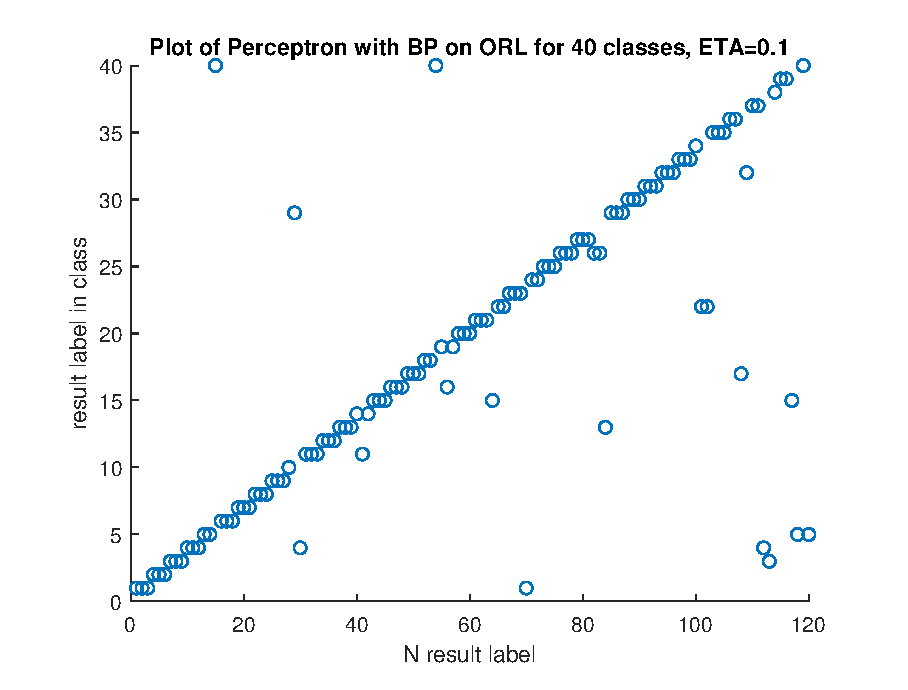
\includegraphics[width=0.7\linewidth]{../ML/results/ORL_Perceptron_BP}}
	\caption{Plot results of training a perceptron with BP on ORL with $\eta=0.1$.}
	\label{fig:orlperceptronbp}
\end{figure}

\begin{figure}[H]
	\centering
	\frame{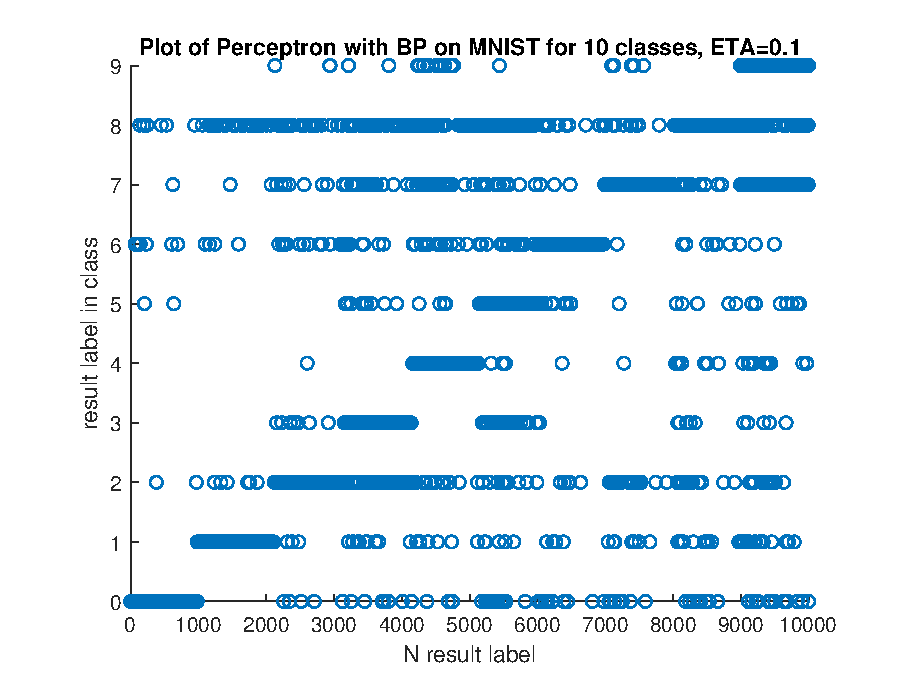
\includegraphics[width=0.7\linewidth]{../ML/results/MNIST_Perceptron_BP}}
	\caption{Plot results of training a perceptron with BP on MNIST with $\eta=1$.}
	\label{fig:mnistperceptronbp}
\end{figure}

\begin{figure}[H]
	\centering
	\frame{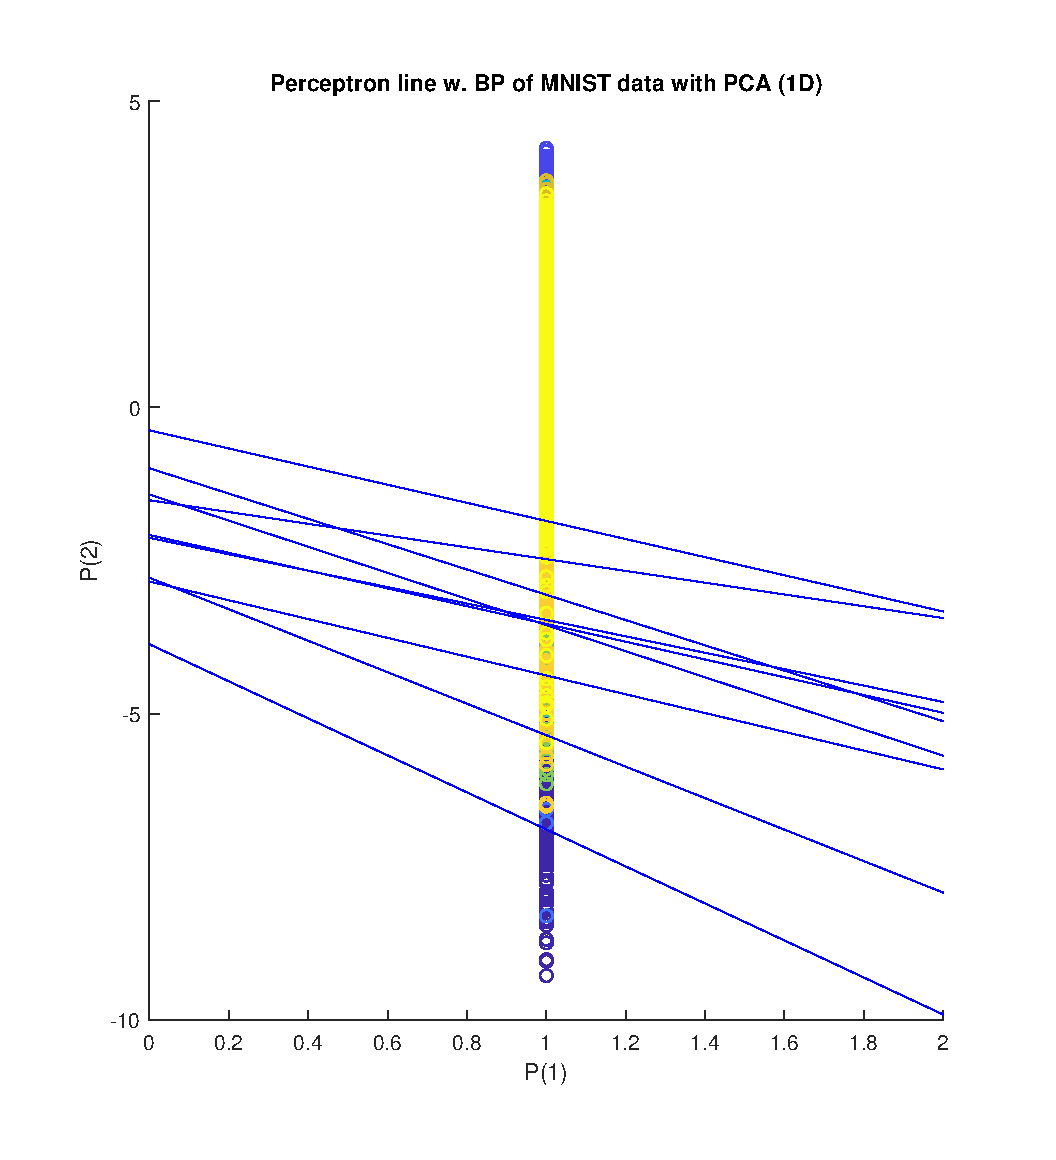
\includegraphics[width=0.7\linewidth]{../ML/results/MNIST_PerceptronLine_BP_1D_PCA}}
	\caption{Plot lines of perceptron with BP for classes on MNIST in 1D.}
	\label{fig:mnistperceptronlinebp1dpca}
\end{figure}

\begin{figure}[H]
	\centering
	\frame{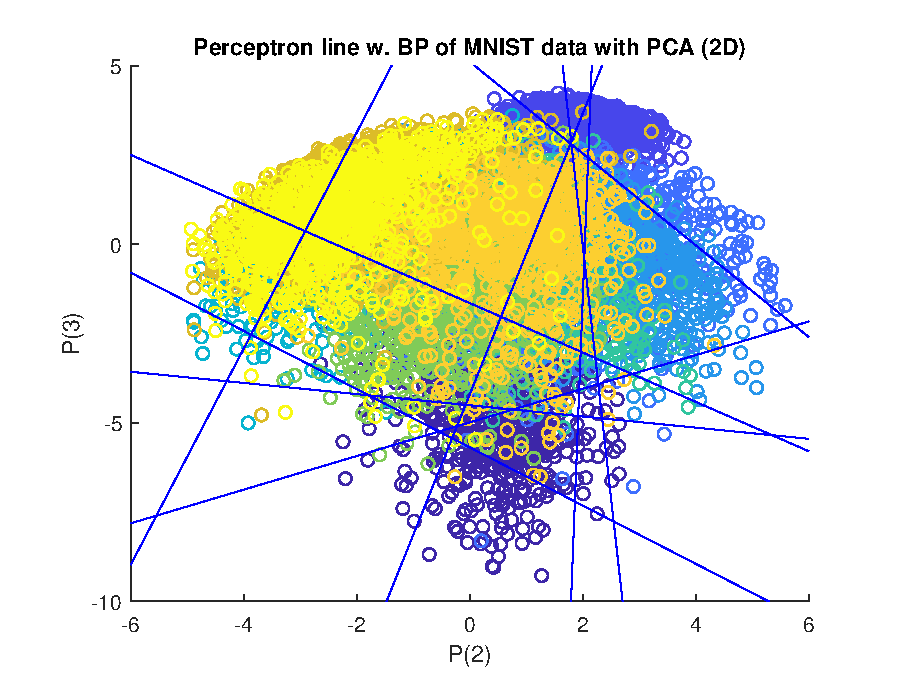
\includegraphics[width=0.7\linewidth]{../ML/results/MNIST_PerceptronLine_BP_2D_PCA}}
	\caption{Plot lines of perceptron with BP for classes on MNIST in 2D.}
	\label{fig:mnistperceptronlinebp2dpca}
\end{figure}

\subsection{Perceptron with MSE}

A perceptron using least-squares was trained on both data sets. Like with backpropagation, we find the class that maximize the decision function $y = w(k)*x_{i}$ for each sample and classify it to that class. Table \ref{table:perceptronmse} details the results, figure \ref{fig:orlperceptronmse} and \ref{fig:mnistperceptronmse} shows plots with the resulting labels.

\begin{table}[H]
	\centering
	\begin{tabular}{|l|l|l|} \hline
		Data set & \pbox{18cm}{Accuracy in $\%$} & \pbox{18cm}{Execution time in $s$} \\ \hline
		ORL & 90\% & 0.05 \\ \hline
		ORL w. PCA & 10\% & 0.01 \\ \hline
		MNIST & 86\% & 6.79 \\ \hline
		MNIST w. PCA & 18.4\% & 0.53 \\ \hline
	\end{tabular}
	\caption{Results for a perceptron with least-squares (MSE) performed on ORL and MNIST.}
	\label{table:perceptronmse}
\end{table}

\begin{figure}[H]
	\centering
	\frame{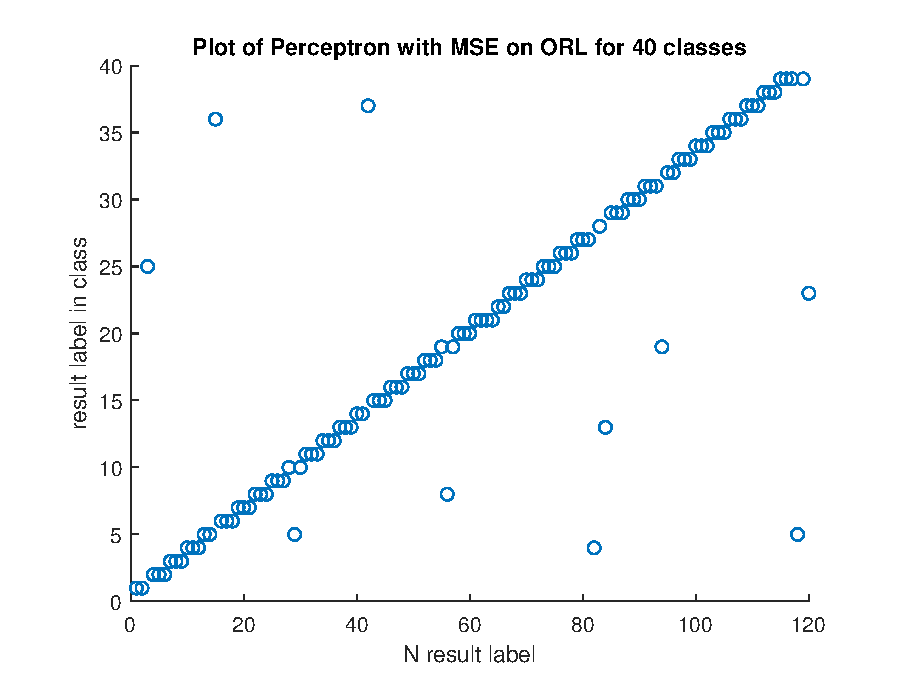
\includegraphics[width=0.7\linewidth]{../ML/results/ORL_Perceptron_MSE}}
	\caption{Plot results of training a perceptron with least-squares (MSE) on ORL.}
	\label{fig:orlperceptronmse}
\end{figure}

\begin{figure}[H]
	\centering
	\frame{\frame{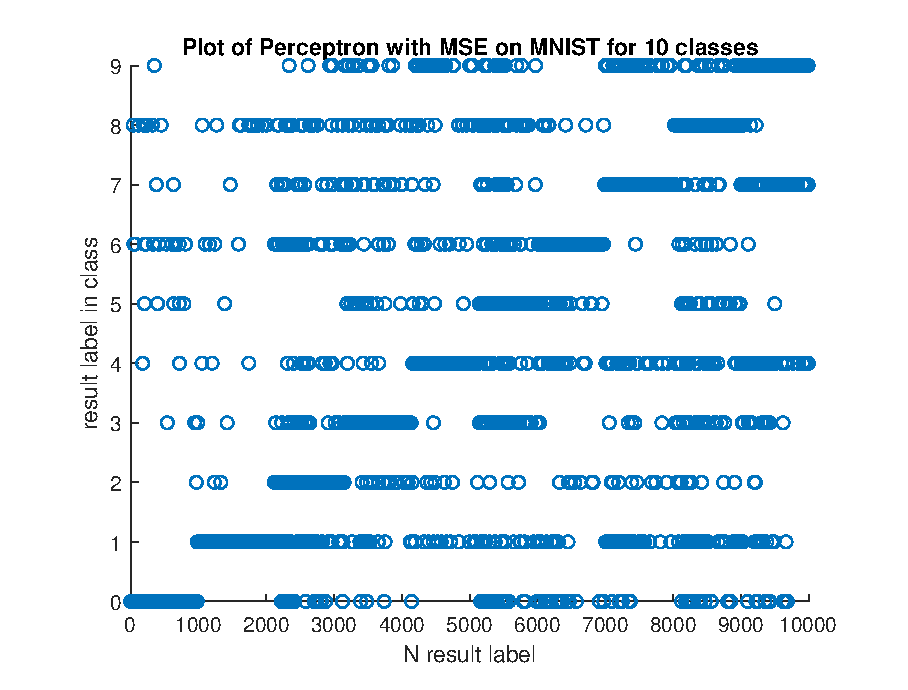
\includegraphics[width=0.7\linewidth]{../ML/results/MNIST_Perceptron_MSE}}}
	\caption{Plot results of training a perceptron with least-squares (MSE) on MNIST.}
	\label{fig:mnistperceptronmse}
\end{figure}

\section{Discussion}

As expected, the algorithms performed differently given the complexity and dimensionality of the data set. If a classification scheme is fast and accurate on a small data set, like ORL ($D=1200$), it might not replicate on a larger set like MNIST ($D=60000$). PCA showed a computational easy way to reduce dimensionality, but accuracy with PCA data lacked in all our tests, averaging around 15\%, even though the execution times were similar to that of the full dimensional sets. Nearest Centroid Classifier (NSC) gained an impressive accuracy on ORL (94.1\%), but struggled on MNIST (75.2\%). Nearest Subclass Centroid (NSC) proved high classification precision, with a 2\% difference between 2 and 5 subclasses on ORL, and 3.9\% on MNIST, however execution times doubled on MNIST with five subclasses compared to just two. Nearest Neighbor (NNC) gave us the best results in terms of accuracy (95.8\% and 96.9\%), but suffered from very high execution times. Our perceptron with BP showed that a lower learning rate $\eta < 0.01$ gave better accuracy with similar execution times as tests with higher learning rate $\eta > 1$. The perceptron performed faster than nearest neighbor (around 2 and 11 minutes on MNIST, respectively) with similar accuracy, showing that a perceptron should be preferred over NNC on larger data sets. The one using least-squares (MSE) gave a sound accuracy on both sets, lower execution times and is a much more simple algorithm to implement and comprehend, though solving the generalized inverse often requires plenty computational resources.

\section{Conclusion}

In this report we have explained the workings of five common classification algorithms including principal component analysis (PCA), the mathematics behind them and benchmarked them on two famous data sets, the ORL set containing 40 different types of facial images and the MNIST set featuring images of numbers from zero to nine. We found that simple algorithms like nearest neighbor classifier (NNC) performs excellent on simple data sets with low dimensionality (like ORL), but struggles on more complex sets like MNIST. In such case, we found that a perceptron trained either by backpropagation or MSE is more suited because it is computational more cost effective, given a boundary is set on number of convergence attempts.

\bibliographystyle{plainnat}
\bibliography{literature}

\end{document}